\section*{Zusammenfassung}

Krebszellen können sich vom Primärtumor lösen und das umgebende Gewebe abbauen. 
Kontinuierliche mathematische Modelle wurden in der Vergangenheit mehrmals verwendet, 
um diesen Prozess besser zu verstehen. In diesem Zusammenhang basiert das Modell 
in der Regel auf mindestens drei Schlüsselkomponenten: den Tumorzellen, dem umgebenden 
Gewebe oder der extrazellulären Matrix (ECM) und den matrixabbauenden Enzymen (MDE). 
Frühe Beschreibungen dieses Modelltyps finden sich in den Arbeiten von Anderson et al. \cite{anderson_continuous_1998,anderson_mathematical_2000} 
und Chaplain et al. \cite{anderson_continuous_1998,chaplain_mathematical_2006,chaplain_mathematical_2006-1,franssen_mathematical_2019}. 
Das zugrunde liegende Modell wird wie folgt beschrieben.
Seien $c$, $e$ und $m$ die Dichte der Tumorzellen, die Dichte der extrazellulären 
Matrix (ECM) und die Konzentration der matrixabbauenden Enzyme (MDE) jeweils. Dann 
lauten die maßgeblichen Gleichungen:

\begin{align*}
	\frac{\partial c}{\partial t} &= D_c \Delta c - \chi \nabla \cdot (c\nabla e) + \mu_1 c\left(1-\frac{c}{c_0}-\frac{e}{e_0}\right)\\
	\frac{\partial e}{\partial t} &= -\delta m e  + \mu_2 c\left(1-\frac{c}{c_0}-\frac{e}{e_0}\right)\\
	\frac{\partial m}{\partial t} &= D_m¸ \Delta c + \mu_3 c - \lambda m
\end{align*}
mit zero-flux Randbedingungen. 
\begin{align*}
	n\cdot (-D_c \nabla c + c \chi\nabla f) &= 0 \\
	n \cdot (-D_m\nabla m ) &= 0
\end{align*}

%\newgeometry{left=20.0mm, right=40.0mm, top=20mm, bottom=20mm, headheight=45mm,  footskip= 12mm, headsep=6mm, marginparsep=0mm}
\noindent Hier sind $D_c$ und $D_m$ die Diffusionskoeffizienten, $\chi$ ist der 
positive haptotaktische Koeffizient, $\delta$ ist eine positive Konstante, und 
$\mu_1$, $\mu_2$, $\mu_3$ sowie $\lambda$ sind die Produktions- und Zerfallskonstanten. \newline
Die Analyse dieses Modells wird in der Literatur größtenteils in $1D$ durchgeführt, 
und einzelne Beispiele wurden in $2D$ gemacht. Allerdings zeigen vorläufige 
Reproduktionen des Modells, dass höhere Dimensionen signifikant unterschiedliche 
Ergebnisse liefern, wie in Abbildung \ref{fig:fig1} zu sehen ist.

\begin{figure}[!h]
 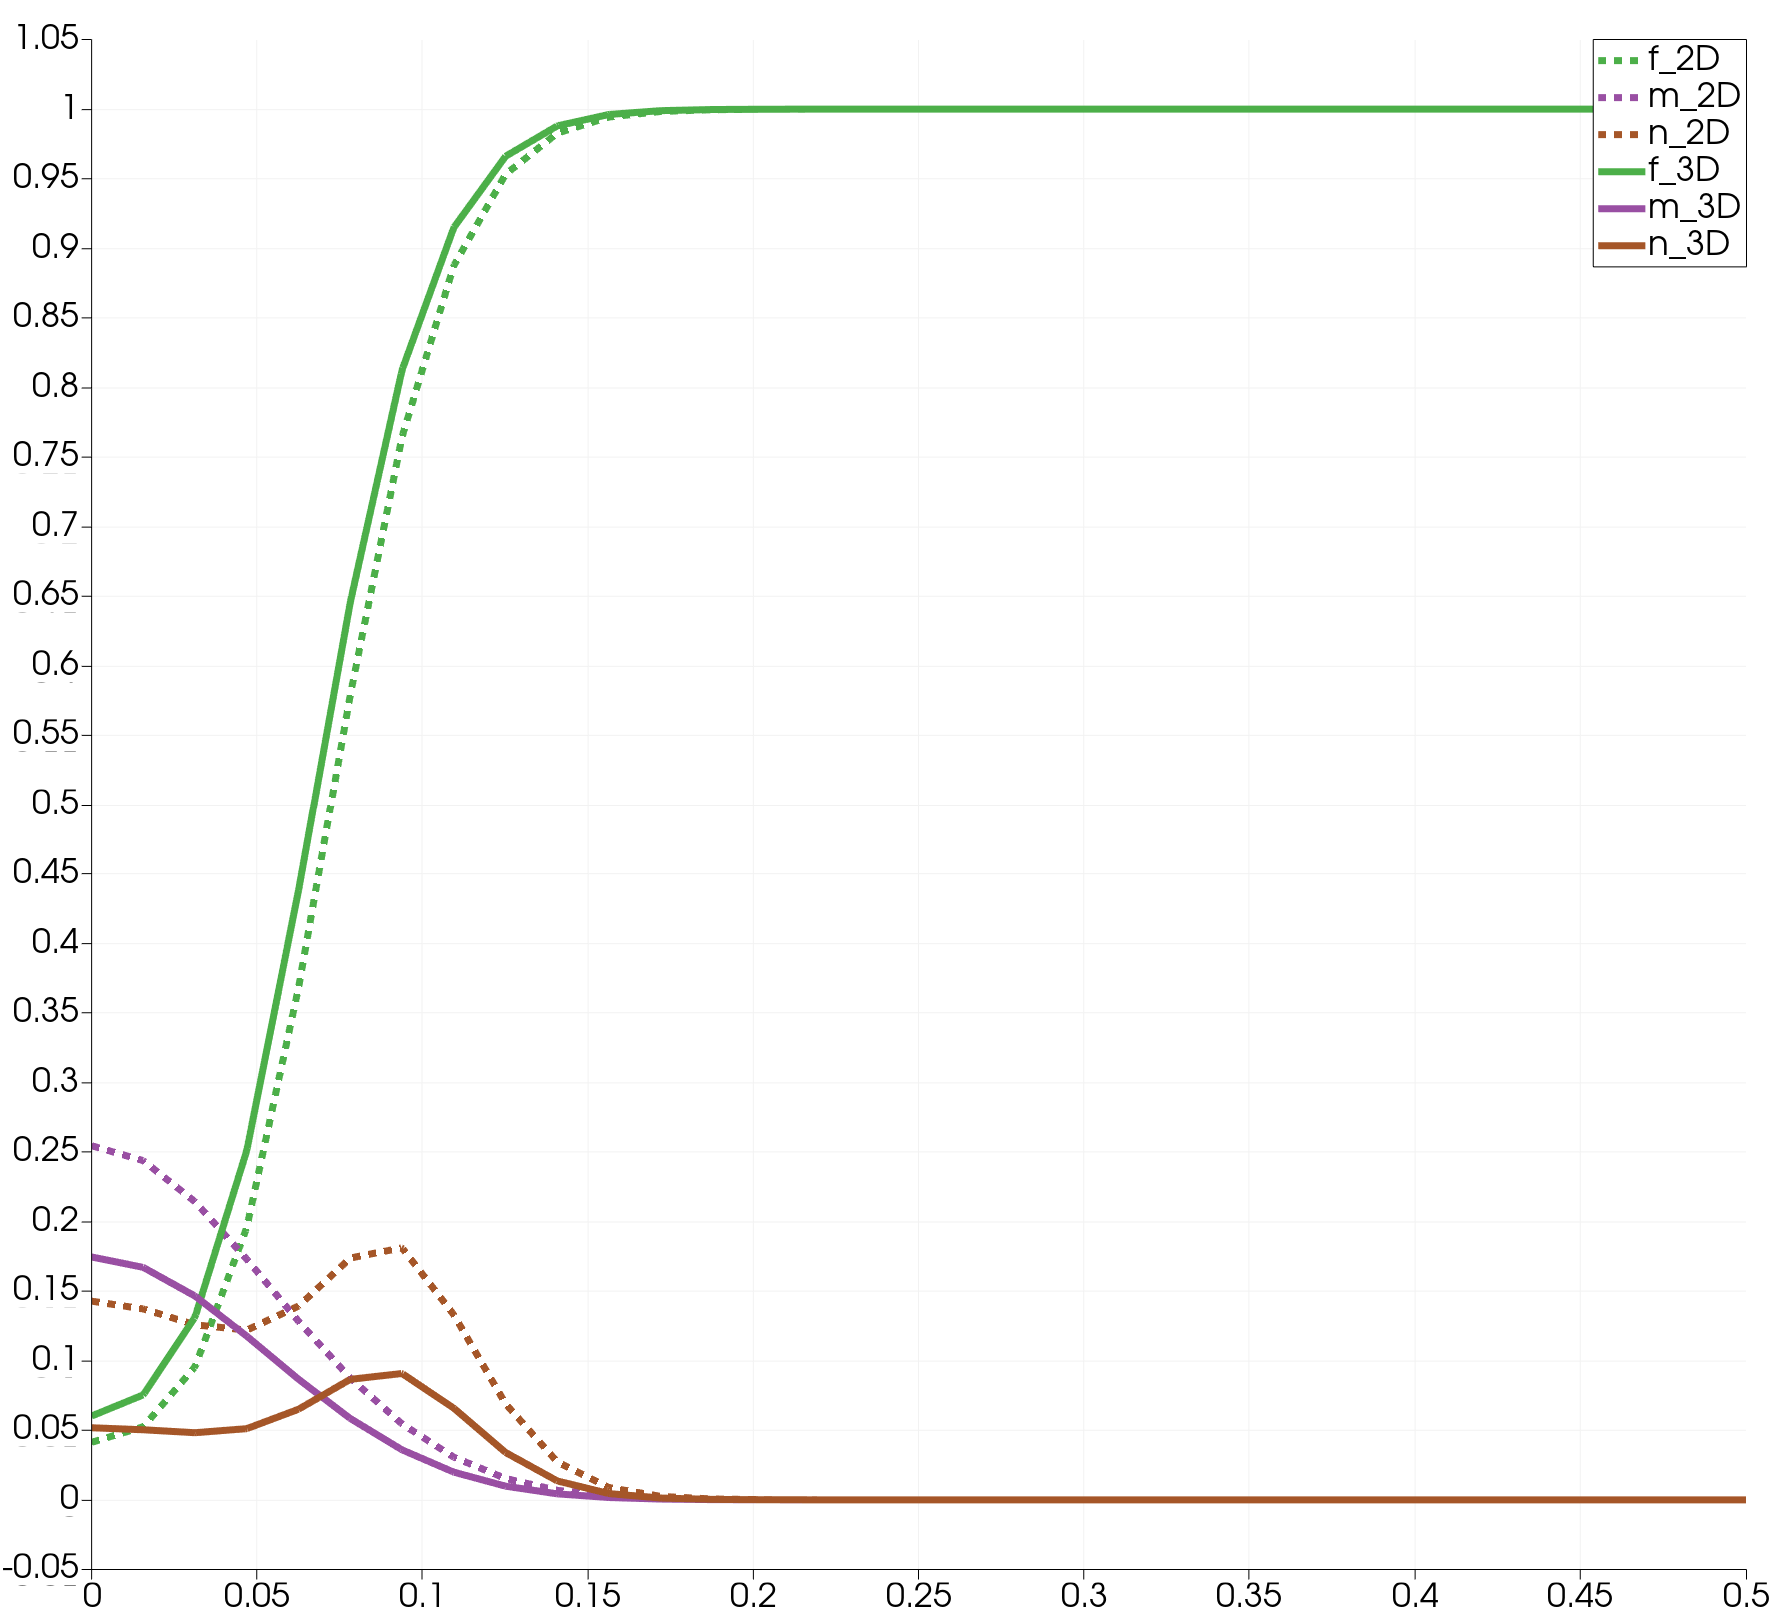
\includegraphics[width=0.45\textwidth]{y/anderson_tumor_invasion_model_2Dvs3Dtime0_7_thick.png}
 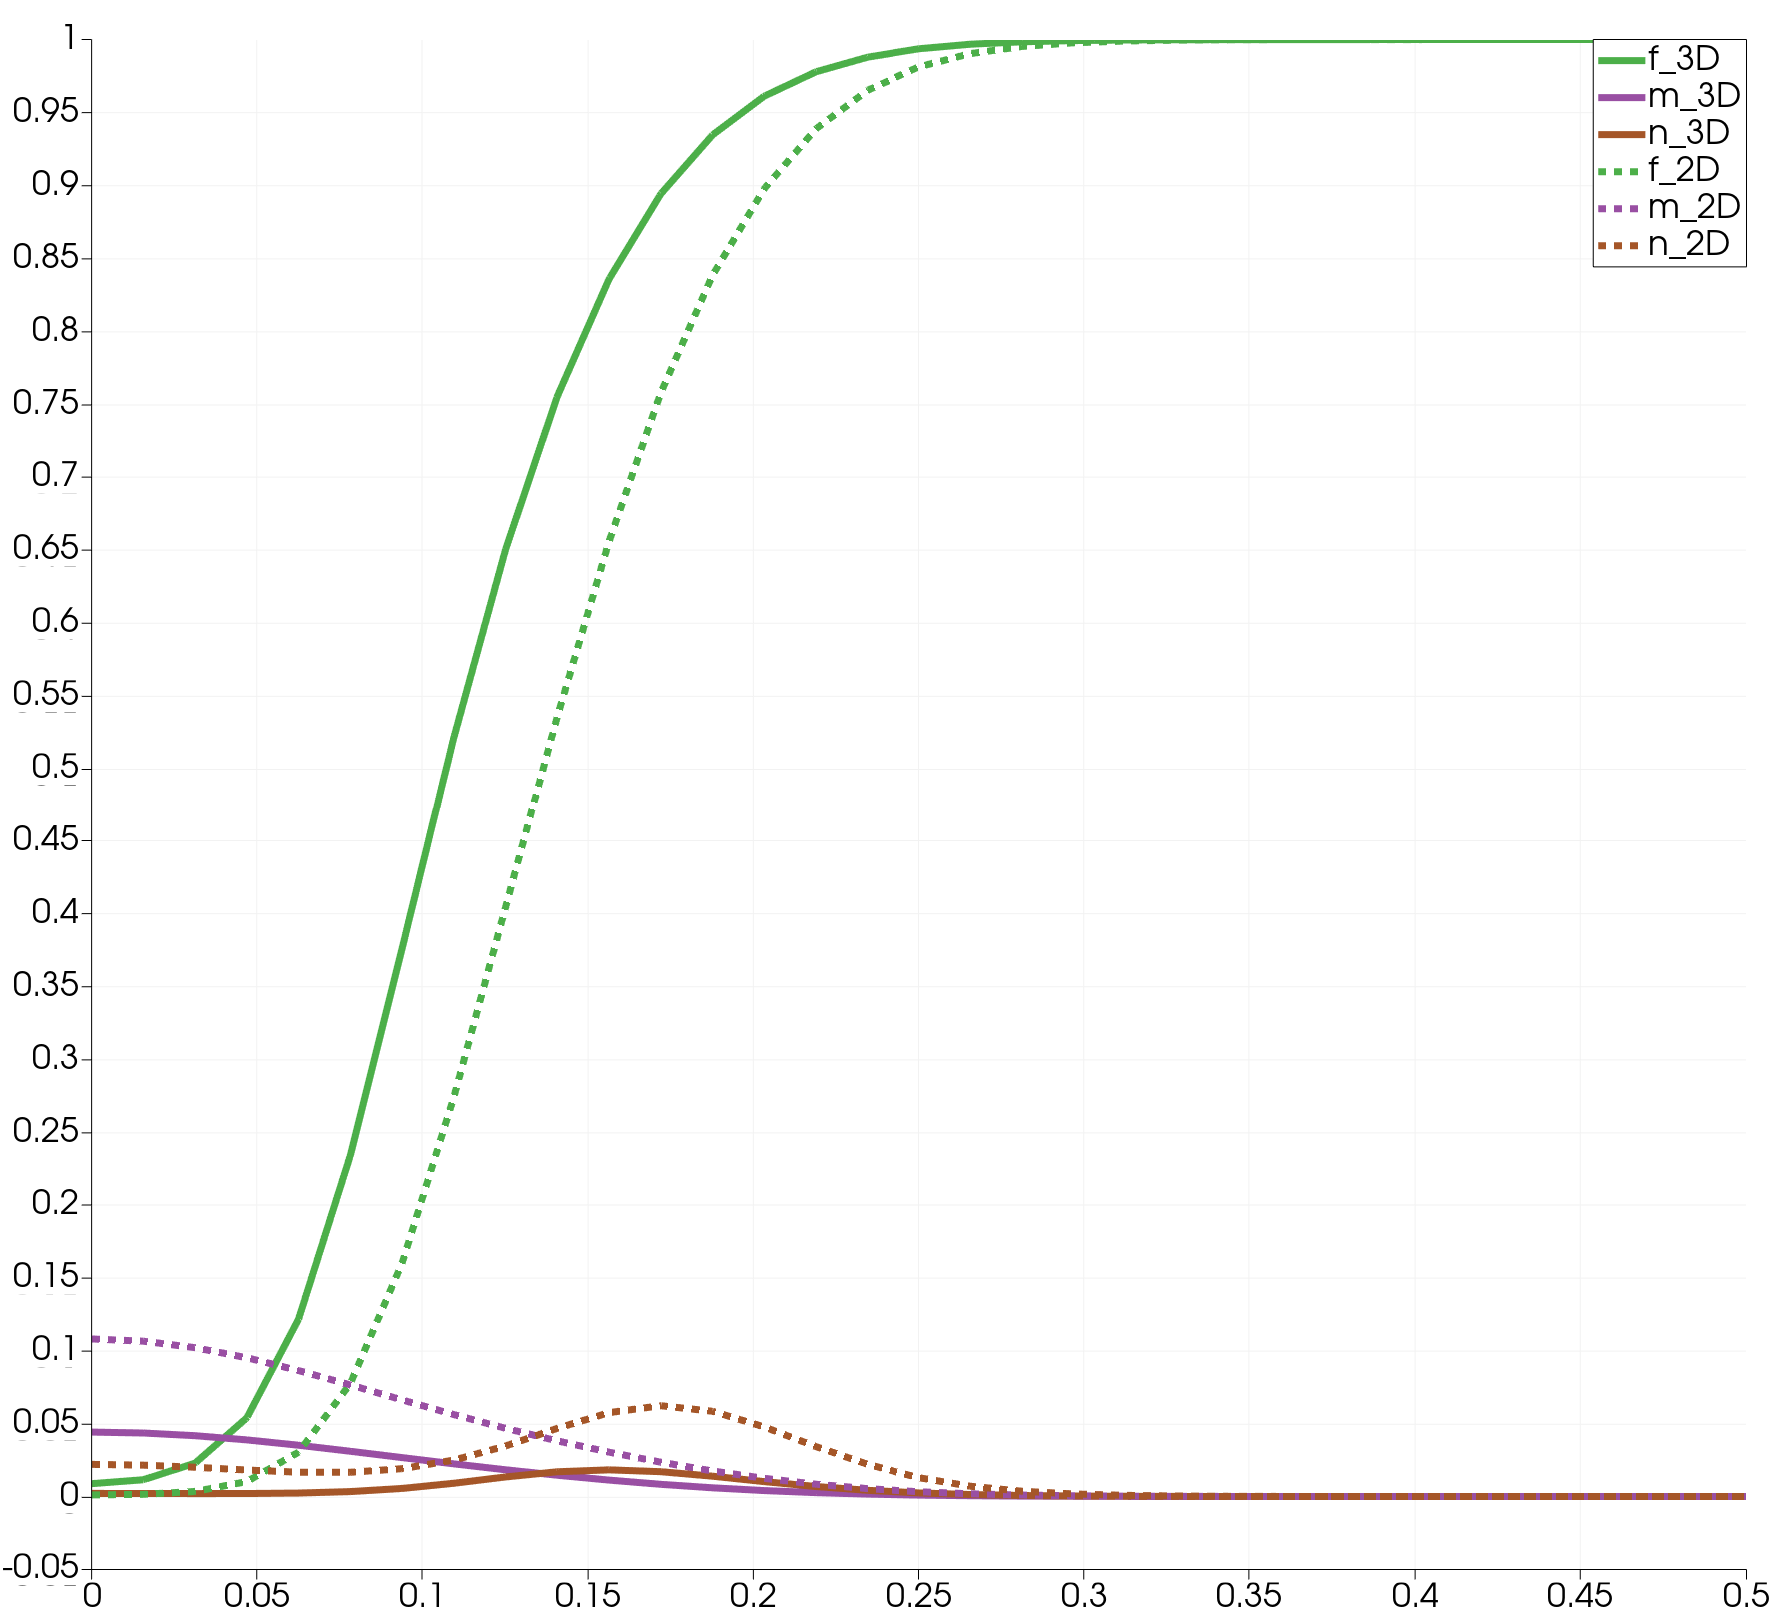
\includegraphics[width=0.45\textwidth]{y/anderson_tumor_invasion_model_2Dvs3D_time3_thick.png}
 \caption{Vorlaeufige Simulationsergebnisse in 2D and 3D des oben beschriebenen Models 
 zur dimensionslosen Zeit $t=0.7$ und $t=3$ sowie den Parametern $D_c=D_m=1e-3$, 
 $\chi=5e-3$, $\delta=10$, $\mu_3=0.1$ und $\lambda=\mu_1=\mu_2 = 0$.}
 \label{fig:fig1}

\end{figure}
Daher stellt sich die Frage, ob die Parameter für dieses Modell für Simulationen in 
$2D$ oder $3D$ unterschiedlich ausgewählt werden müssen oder ob die Ergebnisse und 
Analysen für den eindimensionalen Fall inkorrekt sind. \newline
Darüber hinaus wurde in der Literatur die heterogene Struktur der extrazellulären 
Matrix (ECM) bereits behandelt. Die Struktur der epithelialen Schicht und der 
benachbarten extrazellulären Matrix ist jedoch in biologischem Gewebe organisierter 
als in den gezeigten Simulationen und anderen Beispielen. Daher könnten einfachere 
Unterteilungen der Geometrie in ECM-Gewebe aussagekräftigere Ergebnisse liefern. \newline
Das Ziel dieser Arbeit ist es, einerseits die Parameter und das Modell für höhere 
Dimensionen zu untersuchen und andererseits eine einfache Heterogenität der ECM-Struktur 
in Betracht zu ziehen.

\clearpage
\section*{Abstract}
Cancer cells can migrate from the primary tumor and degrade the surrounding tissue. 
Continuous mathematical models have been used several times in the past to better 
understand this process. In this context, the model is usually based on at least three 
key species, the tumor cells, the surrounding tissue or extracellular matrix (ECM) and 
the matrix degradative enzymes (MDE). Early descriptions of this model type can be found 
in the work of Anderson et al. \cite{anderson_continuous_1998,anderson_mathematical_2000} 
and Chaplain et al. \cite{anderson_continuous_1998,chaplain_mathematical_2006,chaplain_mathematical_2006-1,franssen_mathematical_2019}. 
The underlying model is described as follows. 
Let $c$, $e$ and $m$ be the tumor cell density, the ECM density and the MDE concentration 
respectively. Then, the governing equations are given by

\begin{align*}
	\frac{\partial c}{\partial t} &= D_c \Delta c - \chi \nabla \cdot (c\nabla e) + \mu_1 c\left(1-\frac{c}{c_0}-\frac{e}{e_0}\right)\\
	\frac{\partial e}{\partial t} &= -\delta m e  + \mu_2 c\left(1-\frac{c}{c_0}-\frac{e}{e_0}\right)\\
	\frac{\partial m}{\partial t} &= D_m¸ \Delta c + \mu_3 c - \lambda m
\end{align*}
with zero-flux boundary conditions 
\begin{align*}
	n\cdot (-D_c \nabla c + c \chi\nabla f) &= 0 \\
	n \cdot (-D_m\nabla m ) &= 0
\end{align*}

%\newgeometry{left=20.0mm, right=40.0mm, top=20mm, bottom=20mm, headheight=45mm,  footskip= 12mm, headsep=6mm, marginparsep=0mm}
\noindent Here, $D_c$ and $D_m$ are the diffusion coefficients, $\chi$ is the positive 
haptotactic coefficient, $\delta$ is a positive constant and $\mu_1$,$\mu_2$,$\mu_3$ and 
$\lambda$ are the production and decay constants. \newline 
The analysis of this models is mostly done in $1D$ in the literature and individual 
examples were done in 2D. However, preliminary reproductions of the model show that 
higher dimensions produce significantly different results, as can be seen in Figure\ref{fig:fig2}.

\begin{figure}[!h]
 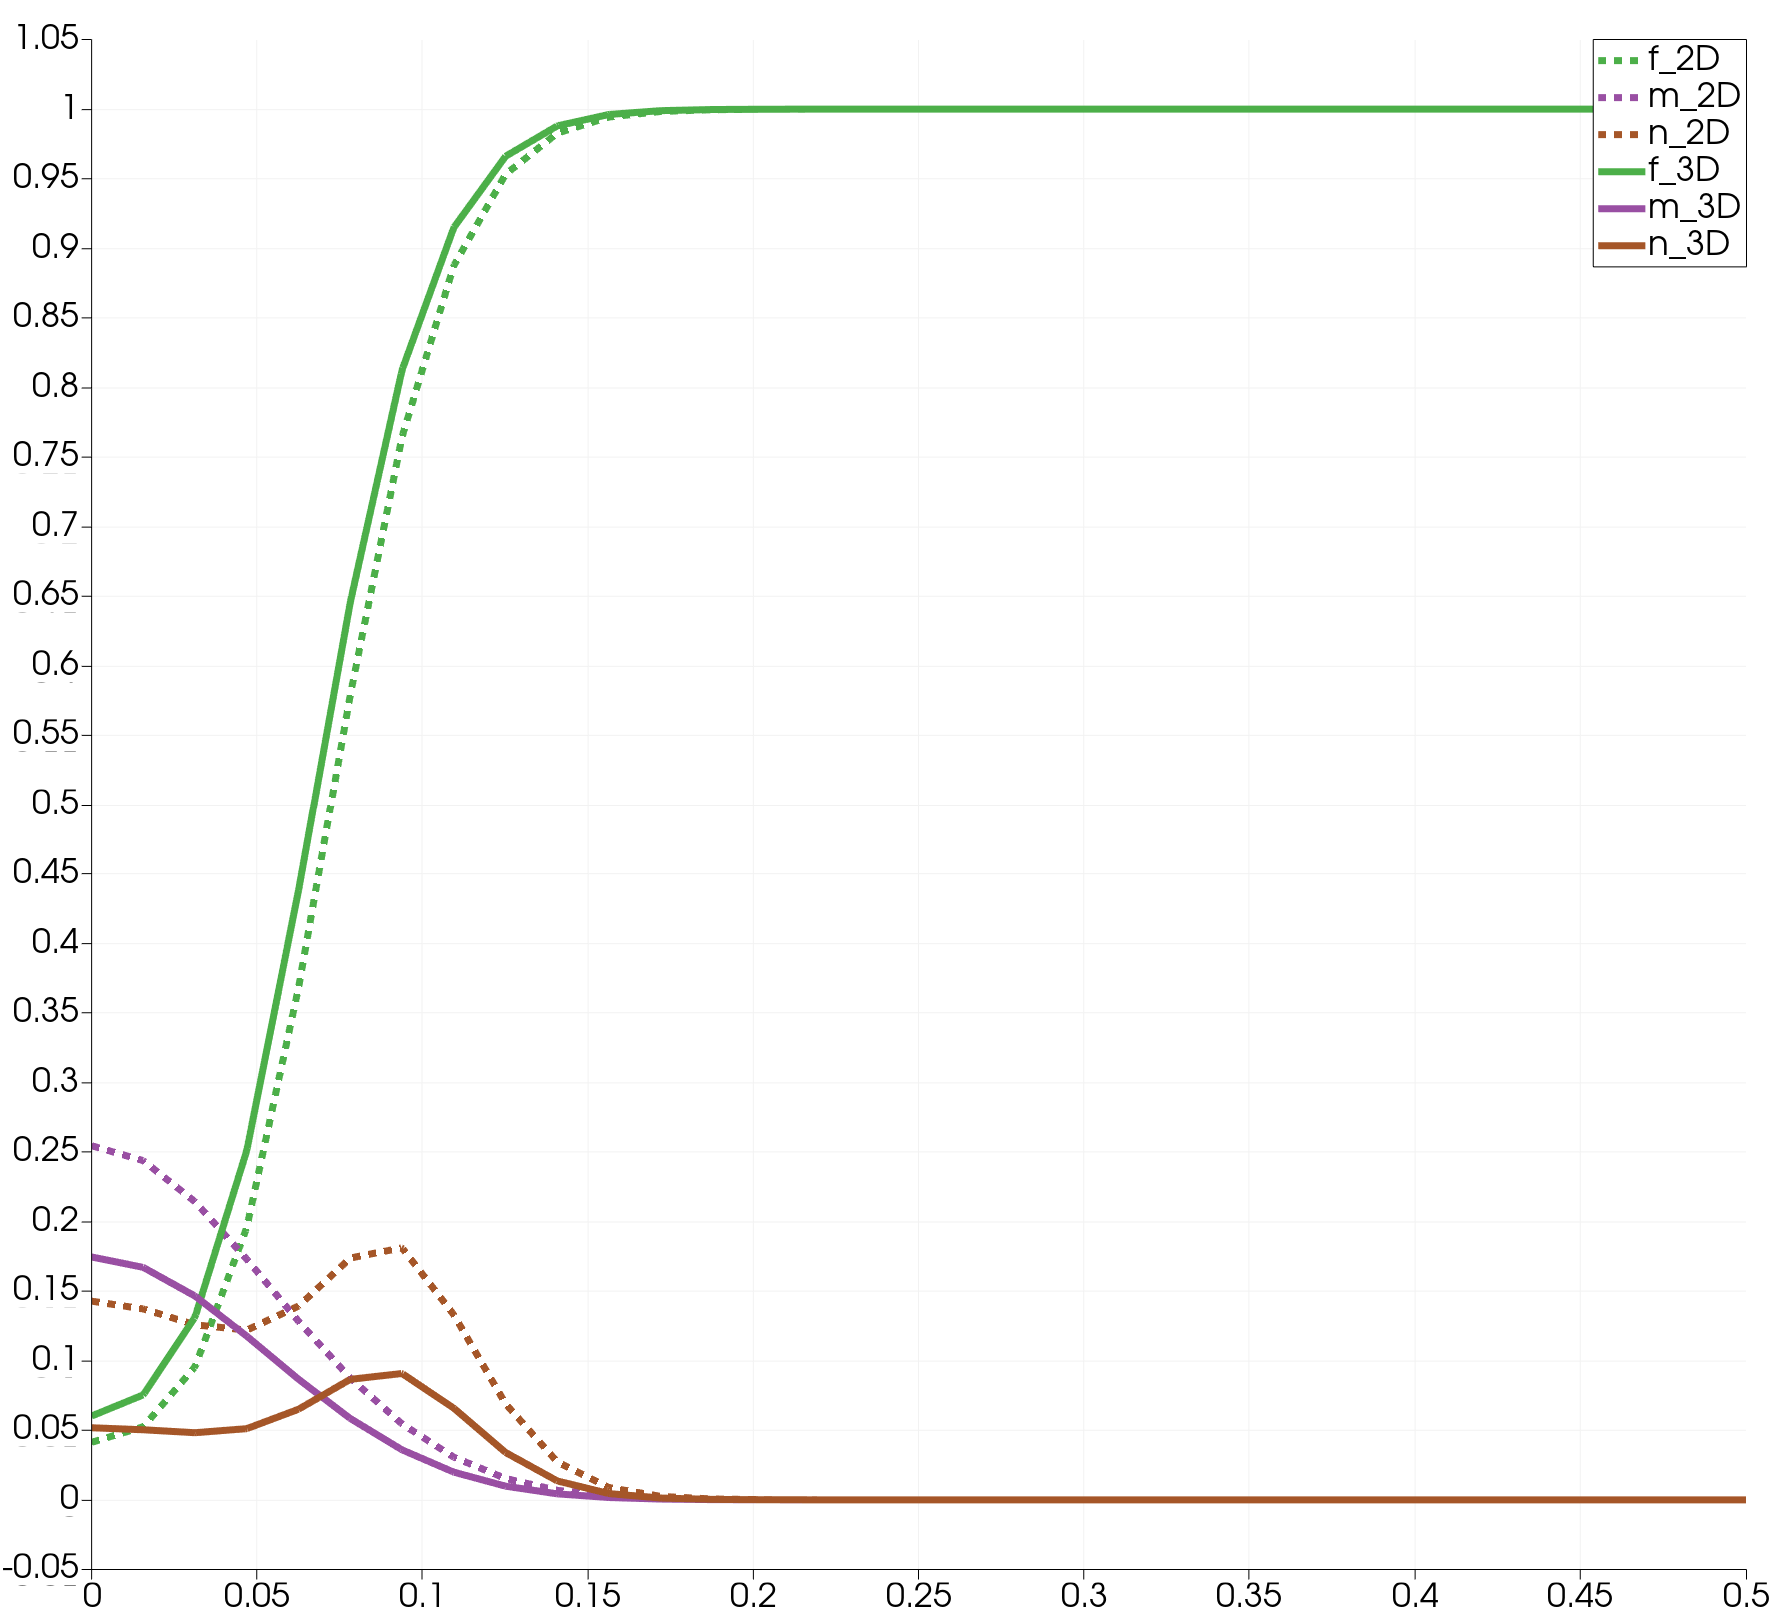
\includegraphics[width=0.45\textwidth]{y/anderson_tumor_invasion_model_2Dvs3Dtime0_7_thick.png}
 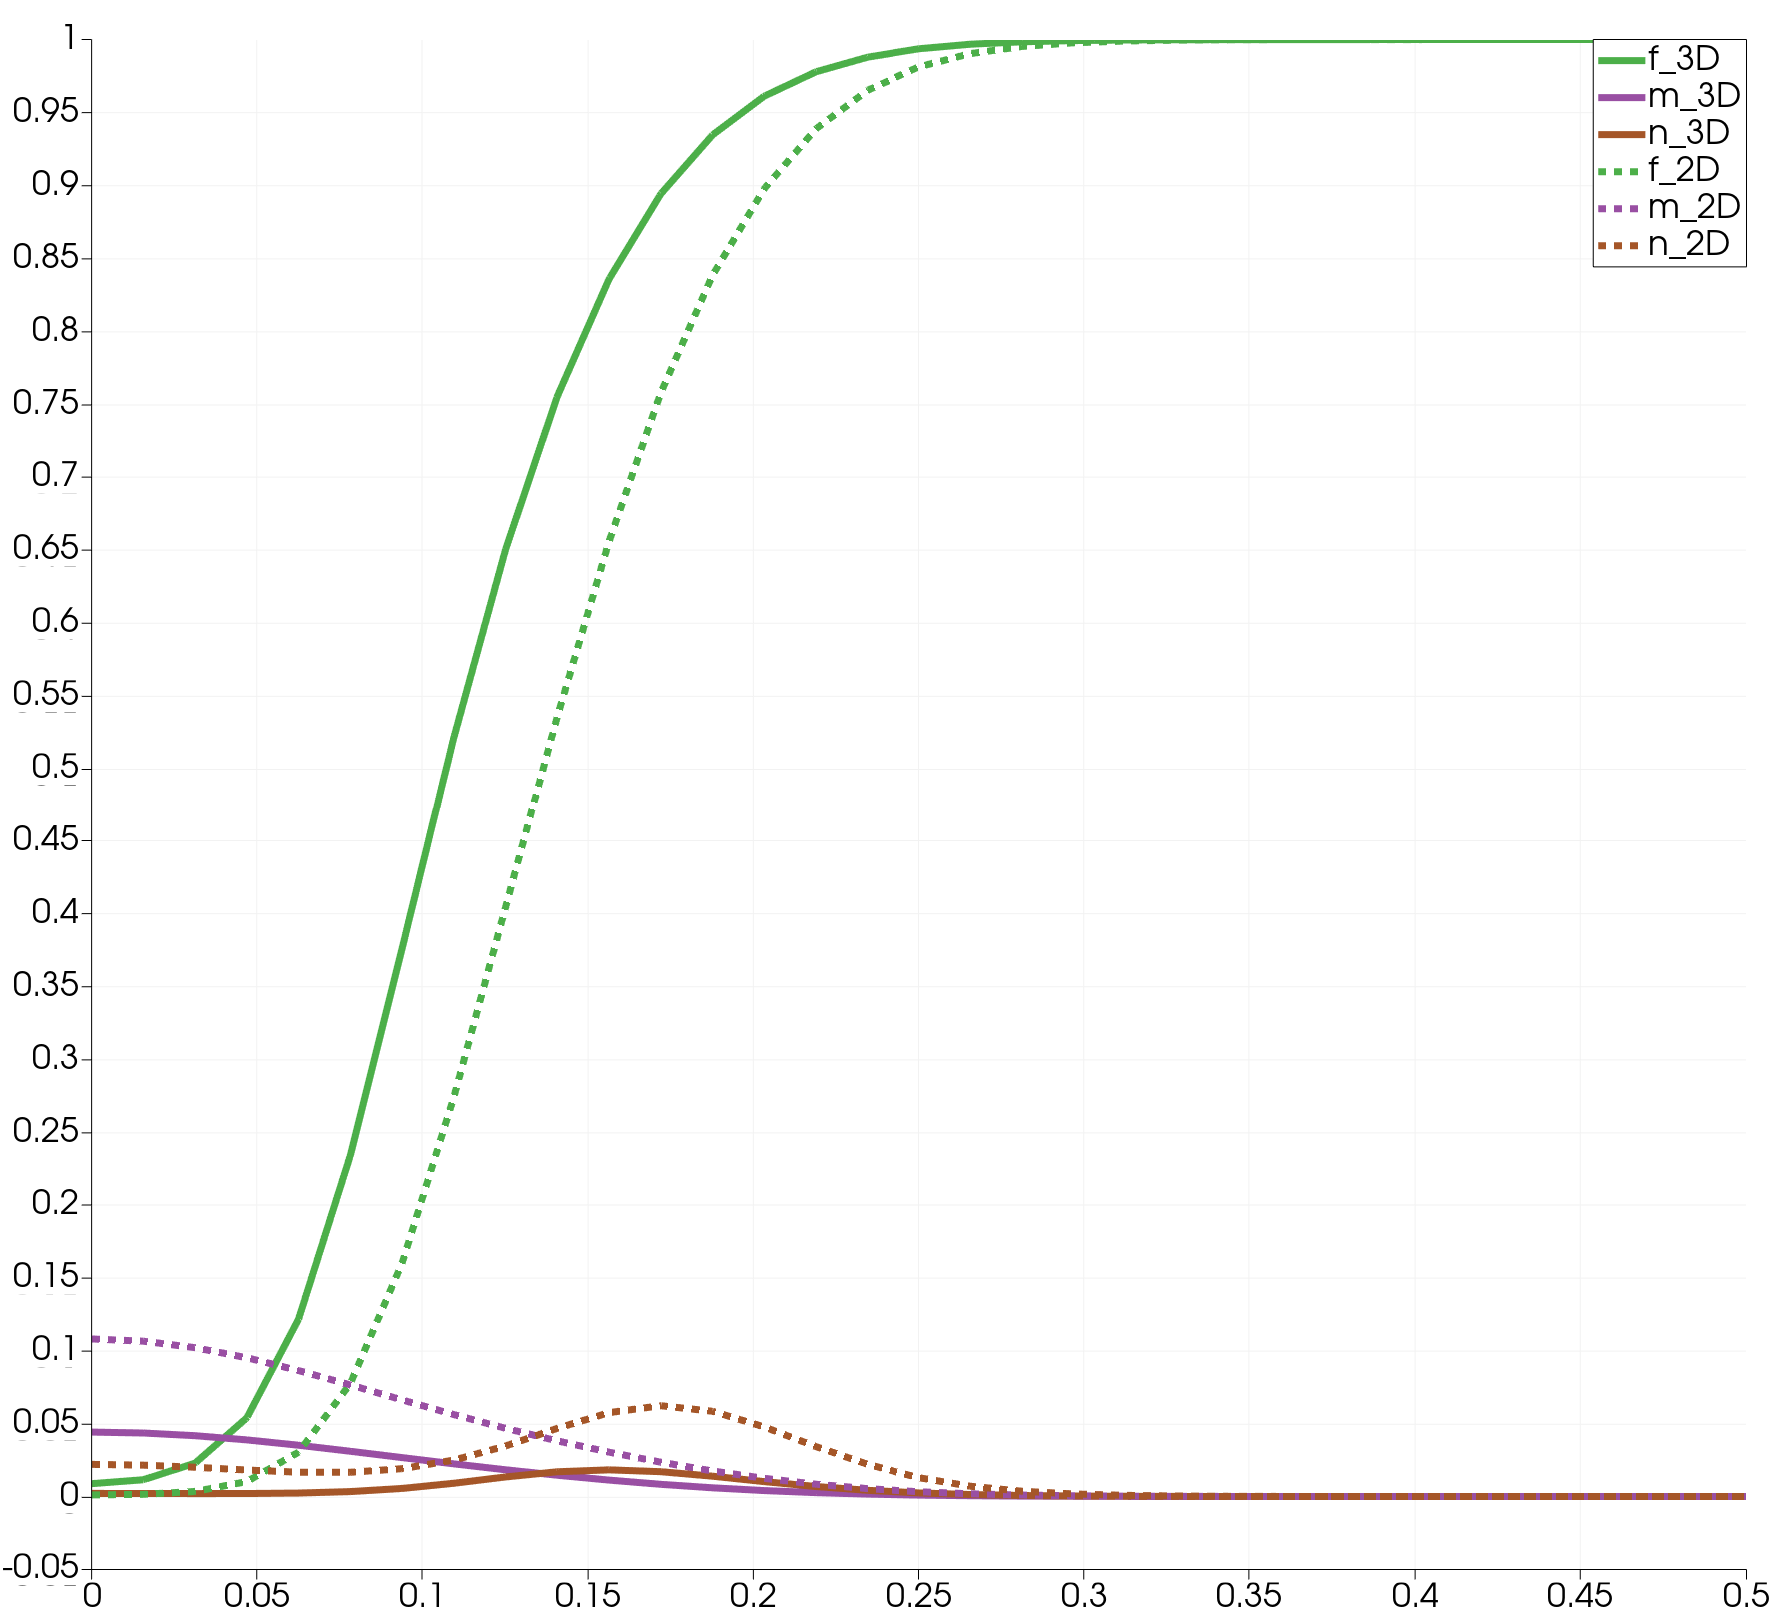
\includegraphics[width=0.45\textwidth]{y/anderson_tumor_invasion_model_2Dvs3D_time3_thick.png}
 \caption{Preliminary simulation results in 2D and 3D of the above described model at dimensionless time $t=0.7$ and $t=3$ and parameters $D_c=D_m=1e-3$, $\chi=5e-3$, $\delta=10$, $\mu_3=0.1$ and $\lambda=\mu_1=\mu_2 = 0$. }
 \label{fig:fig2}

\end{figure}
The question therefore arises as to whether the parameters for this model need to 
be selected differently for simulations in 2D or 3D, or whether the results and 
analysis for the one dimensional case is incorrect. \newline
Furthermore, the heterogeneous ECM structure has been addressed in the literature. 
However, the structure of the epithelial layer and the adjacent extracellular 
matrix is more organized in biological tissue than in the simulations shown in and, 
for example. Therefore, simpler subdivisions of the geometry into ECM tissue could 
provide more meaningful results. \newline
The aim of this work is to investigate the parameters and the model for higher 
dimensions on the one hand, and to consider a simple heterogeneity of the ECM 
structure on the other hand.